\section{Morfeas System Loggers}
The Morfeas System Loggers utility is made to show information related to the Morfeas System's components.
It's can be accessed for the Morfeas WEB front page by the button with this 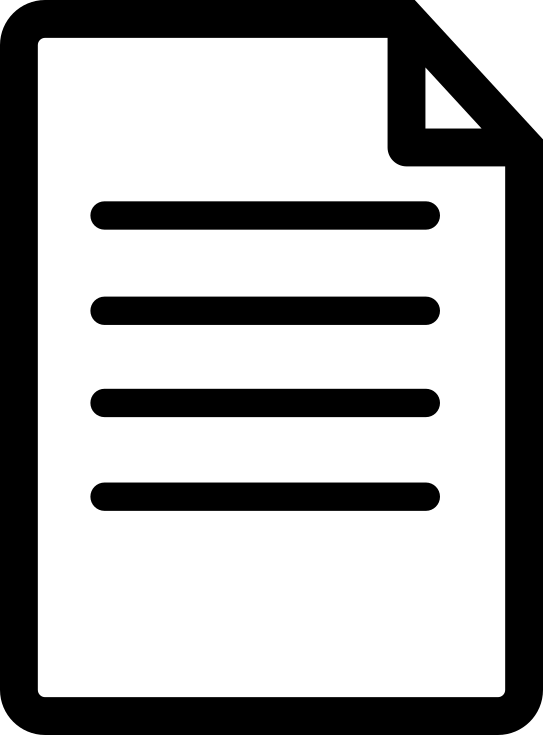
\includegraphics[height=.125in]{../art/logger.png} symbol.
\begin{figure}[h]
\centering
	\fbox{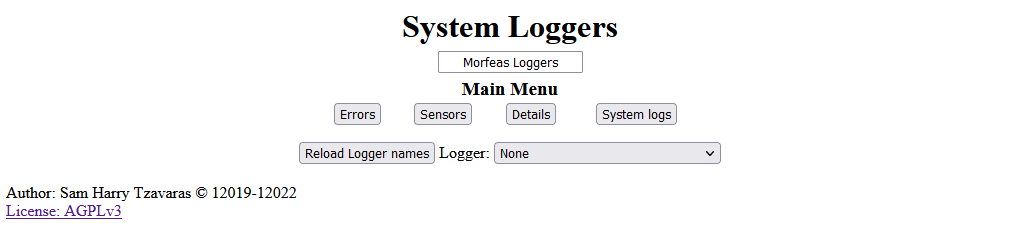
\includegraphics[width=4in]{../art/Morfeas_web_if/Morfeas_system_loggers.png}}
	\caption{Morfeas System Loggers}
	\label{fig:morfeas_loggers}
\end{figure}

At table \ref{tab:morfeas_loggers} present the functionality of the utility's tabs.
\begin{table}[h!]
	\begin{center}
		\begin{tabular}{|c|l|}
			\hline
			\textbf{Tab Name} & \textbf{Purpose}\\
			\hline
			Errors & Table with Sensors that reporting error.\\
			\hline
			Sensors & Table with all the available sensor.\\
			\hline
			Details & Table with report of component's status.\\
			\hline
			System Logs & Loggers from Morfeas' system components (Default).\\
			\hline
		\end{tabular}
		\caption{Morfeas System Loggers values}
		\label{tab:morfeas_loggers}
	\end{center}
\end{table}

The ``System logs" is the tab that shown by default at the opening of the utility.
For the drop-down list at the bottom right it's can be selected the logger of the component on interest.
Each ``Morfeas Component loggers", is a human readable output (ASCI text) of the component.
The ``Reload Logger names" button refresh the list of components, by request from the device server.
The Components of the ``Morfeas system" configured from the ``Morfeas System configuration" utility (section \ref{sys_conf}).\\

The ``Details" tab shows all the status reports from the components.
The ``Sensors" tab present a list of the active sensors from all components.
And the ``Error" all the sensors that reporting error at status.
